\documentclass[../AnalysisNoteJBuxton.tex]{subfiles}
\begin{document}

\subsection{Results: \texorpdfstring{$\Xi$K$^{\pm}$}{TEXT}}
\label{ResultsXiK}

Preliminary results and fits for our $\Xi$K$^{\pm}$ analyses are expected to be uploaded by 16 December 2016.

Even without any fits to the data, the fact that the $\Xi^{-}$K$^{+}$ data dips below unity is exciting, as this cannot occur purely from a Coulomb interaction.  We hope that this dip signifies that we are able to peer through the overwhelming contribution from the Coulomb interaction to see the effects arising from the strong interaction.

\begin{figure}[h]
  \centering
  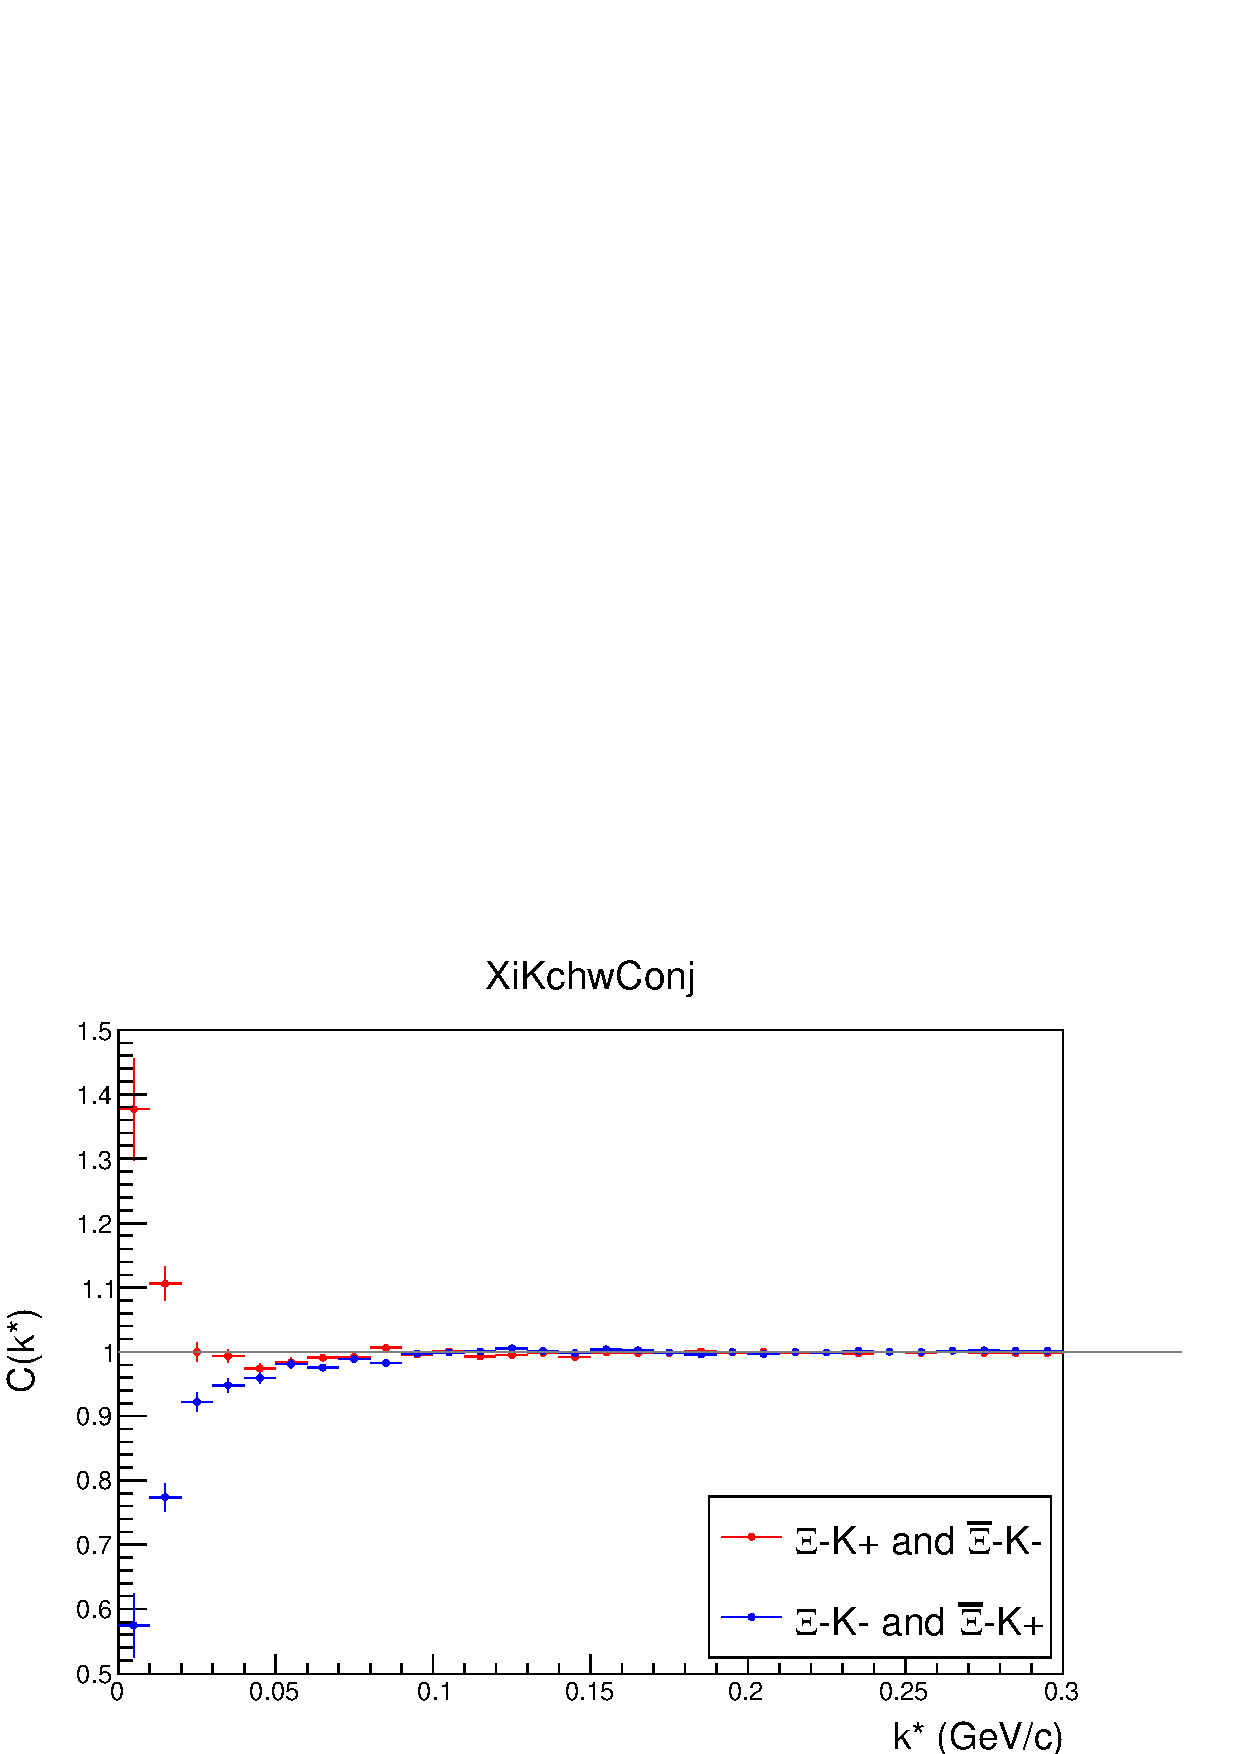
\includegraphics[width=\textwidth]{7_ResultsAndDiscussion/Figures/XiKchwConjKStarCf.pdf}
  \caption[$\Xi$K$^{\pm}$ Results]{$\Xi$K$^{\pm}$ Results for 0-10\% Centrality}
  \label{fig:XiKchwConjResults}
\end{figure}

\begin{figure}[h!]
  \centering
  %%----start of first subfigure---  
  \subfloat[$\Xi$K$^{+}$ First Fit, 0-10\% Centrality]{
    \label{fig:XiKchFits:a}
    \includegraphics[width=0.49\textwidth]{7_ResultsAndDiscussion/Figures/XiKchP.pdf}}
  %%----start of second subfigure---
  \subfloat[$\bar{\Xi}$K$^{+}$ First Fit, 0-10\% Centrality]{
    \label{fig:XiKchFits:b}
    \includegraphics[width=0.49\textwidth]{7_ResultsAndDiscussion/Figures/AXiKchP.pdf}}
  %%----overall caption----
  \caption[$\Xi$K$^{\pm}$ First Fits]{$\Xi$K$^{\pm}$ First Fits}
  \label{fig:XiKchFits}
\end{figure}



\end{document}